\documentclass[11pt,oneside]{article}
\usepackage[T1]{fontenc}
\usepackage[utf8]{inputenc}
%\DeclareUnicodeCharacter{00A0}{ }
\usepackage[adobe-utopia]{mathdesign}

\usepackage{amsmath}
\usepackage[francais]{babel}
\usepackage[dvips]{graphicx}
%\usepackage{here}
\usepackage{framed}
\usepackage[normalem]{ulem}
\usepackage{fancyhdr}
\usepackage{titlesec}
\usepackage{vmargin}

\usepackage{amsmath}
\usepackage{ifthen}
\usepackage{multirow}
\usepackage{multicol} % Portions de texte en colonnes

%\usepackage{xltxtra} % Logo XeLaTeX
%\usepackage{pst-solides3d}
\usepackage{color}
%\usepackage{colortbl}
\usepackage{titletoc} % Pour la mise en forme de la table des matières

%\usepackage[crop=off]{auto-pst-pdf}
%\usepackage{bclogo}


%\usepackage{longtable}
%\usepackage{flafter}%floatants après la référence
%\usepackage{pst-solides3d}
%\usepackage{pstricks}
%\usepackage{minitoc}
%\setcounter{minitocdepth}{4}
%\usepackage{draftcopy}% "Brouillon"
%\usepackage{floatflt}
%\usepackage{psfrag}
%\usepackage{listings} % Permet d'insérer du code de programmation
%\usepackage{lmodern}
%\usepackage[adobe-utopia,uppercase=upright,greeklowercase=upright]{mathdesign}
%\usepackage{minionpro}
%\usepackage{pifont}
%\usepackage{amssymb}
%\usepackage[francais]{varioref}

\setmarginsrb{1.5cm}{1cm}{1cm}{1.5cm}{1cm}{1cm}{1cm}{1cm}

\definecolor{gris25}{gray}{0.75}
\definecolor{bleu}{RGB}{18,33,98}
\definecolor{bleuf}{RGB}{42,94,171}
\definecolor{bleuc}{RGB}{231,239,247}
\definecolor{rougef}{RGB}{185,18,27}
\definecolor{rougec}{RGB}{255,230,231}
\definecolor{vertf}{RGB}{103,126,82}
\definecolor{vertc}{RGB}{220,255,191}
\definecolor{violetf}{RGB}{112,48,160}
\definecolor{violetc}{RGB}{230,224,236}
\definecolor{jaunec}{RGB}{220,255,191}
\usepackage[raccourcis]{FAST}
\usepackage[%
    pdftitle={IS -- SysML -- Diagramme de définiton des blocs},
    pdfauthor={Xavier Pessoles},
    colorlinks=true,
    linkcolor=blue,
    citecolor=magenta]{hyperref}

\usepackage{pifont}


% \makeatletter \let\ps@plain\ps@empty \makeatother
%% DEBUT DU DOCUMENT
%% =================
\sloppy
\hyphenpenalty 10000

\newcommand{\Pointilles}[1][3]{%
\multido{}{#1}{\makebox[\linewidth]{\dotfill}\\[\parskip]
}}


\colorlet{shadecolor}{orange!15}

\newtheorem{theorem}{Theorem}


\begin{document}


\newboolean{prof}
\setboolean{prof}{true}
%------------- En tetes et Pieds de Pages ------------
\pagestyle{fancy}
\renewcommand{\headrulewidth}{0pt}

\fancyhead{}
\fancyhead[L]{%
\noindent\noindent\begin{minipage}[c]{2.6cm}
%Lycée Rouvière PTSI

\includegraphics[width=2cm]{png/logo_ptsi.png}%
\end{minipage}
}


\fancyhead[C]{\rule{12cm}{.5pt}}

\fancyhead[R]{%
\noindent\begin{minipage}[c]{3cm}
\begin{flushright}
\footnotesize{\textit{\textsf{Sciences Industrielles\\ de l'Ingénieur}}}%
\end{flushright}
\end{minipage}
}

\renewcommand{\footrulewidth}{0.2pt}

\fancyfoot[C]{\footnotesize{\bfseries \thepage}}
\fancyfoot[L]{\footnotesize{2013 -- 2014} \\ X. \textsc{Pessoles}}
\ifthenelse{\boolean{prof}}{%
\fancyfoot[R]{\footnotesize{CI 1 : IS -- Cours \\
Ch 4 SysML -- Définition des blocs-- P}}
}{%
\fancyfoot[R]{\footnotesize{Cours -- CI 6 : PPM}}
}



\begin{center}
 \huge\textsc{CI 1 -- IS}

 \large\textsc{Étude des systèmes pluritechniques et multiphysiques -- Initiation à l'Ingénierie Système}
\end{center}

\begin{center}
 \LARGE\textsc{Chapitre 4 -- SysML -- Diagramme de définition des blocs}
\end{center}

%\begin{flushright}
%\textit{D'après documents de Jean-Pierre Pupier}
%\end{flushright}

\vspace{.5cm}


\begin{savoir}
\textsc{Savoirs}
\begin{itemize}
\item A-C3.1 : Analyse structurelle et comportementale
\end{itemize}
\end{savoir}

Le diagramme des blocs permet de présenter et de détailler les différents constituants d'un système.
\begin{center}
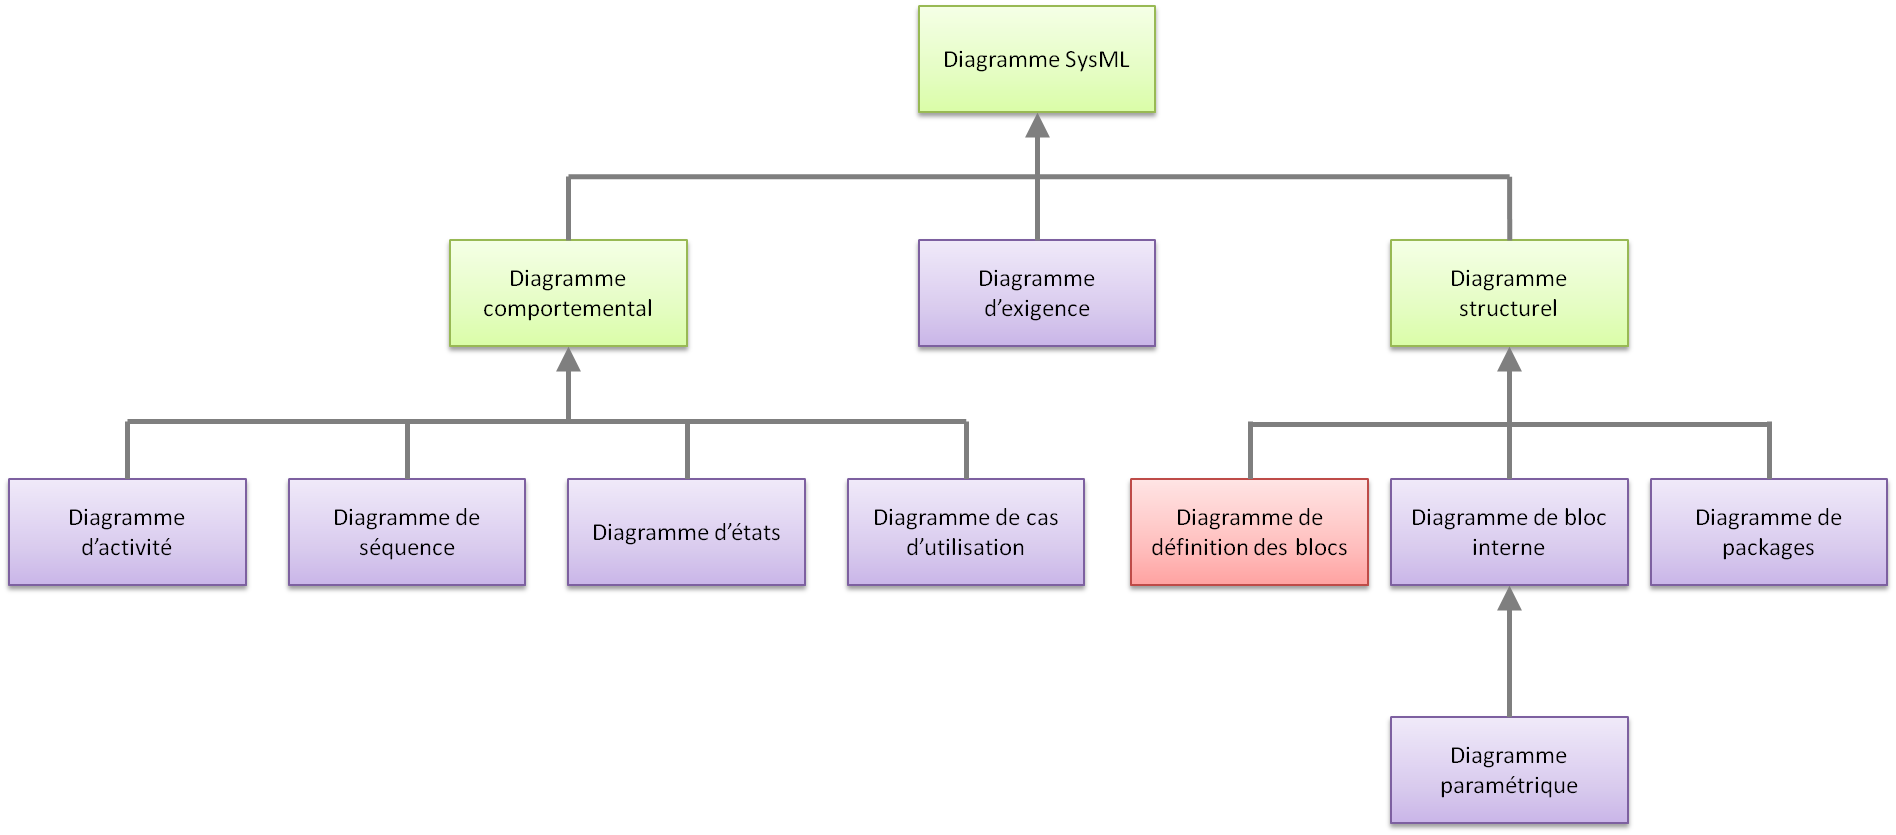
\includegraphics[width=\textwidth]{png/def_blocs}
\end{center}
 
\setlength{\parskip}{0ex plus 0.2ex minus 0ex}
 \renewcommand{\contentsname}{}
 \renewcommand{\baselinestretch}{1}

\tableofcontents

 \renewcommand{\baselinestretch}{1.2}
\setlength{\parskip}{2ex plus 0.5ex minus 0.2ex}

% \vspace{1cm}
\textit{Ce document évolue. Merci de signaler toutes erreurs ou coquilles.}

\section{Présentation}

\begin{defi}
\begin{minipage}[c]{.7\linewidth}
\textbf{Bloc} --  \textit{Block}

Un bloc représente un système ou un de ses composants. On peut y renseigner diverses propriétés et y associer une image, un lien ou tout autre document. 
\end{minipage}\hfill
\begin{minipage}[c]{.25\linewidth}
\begin{center}
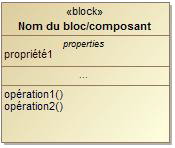
\includegraphics[width=.9\textwidth]{png/block}
\end{center}
\end{minipage}
\end{defi}

\begin{defi}
\textbf{Liens entre blocs}

Chaque bloc peut être relié avec d'autres blocs ou avec des acteurs :
\begin{itemize}
\item \textbf{la composition} indique que le bloc 2 appartient au bloc 1 (le bloc 2 est une partie du bloc 1);
\item \textbf{l'association} indique un lien entre blocs mais sans contenance. 
\end{itemize}

\begin{minipage}[c]{.45\linewidth}
\begin{center}
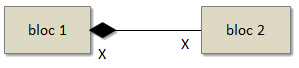
\includegraphics[width=.9\textwidth]{png/composition}

\textit{Composition}
\end{center}
\end{minipage}\hfill
\begin{minipage}[c]{.45\linewidth}
\begin{center}
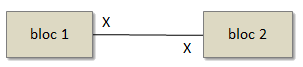
\includegraphics[width=.9\textwidth]{png/association}

\textit{Association}
\end{center}
\end{minipage}
\end{defi}

\begin{rem}
\textit{Multiplicité}

$X$ indique la multiplicité du bloc, c’est-à-dire le nombre d’instances du bloc vérifiant la relation (plusieurs est noté *).
\end{rem}

\begin{defi}
\textbf{Diagramme de définition des blocs} --  \textit{Block Diagram Definition}

Ce diagramme permet de représenter les différents constituants d’un système, ainsi que les liens entre eux. Il montre ainsi la structure du système.
\end{defi}

\begin{exemple}
\begin{center}
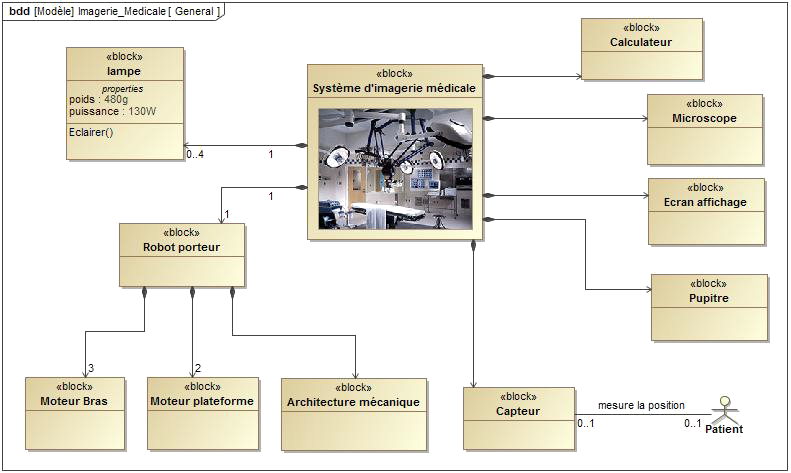
\includegraphics[width=.9\textwidth]{png/exemple}
\end{center}
\end{exemple}

\begin{thebibliography}{2}
\bibitem{roques}{Pascal Roques, SysML par l'exemple -- Un langage de modélisation pour systèmes complexes. Éditions Eyrolles, 2009.}
\bibitem{debout}{Pierre Debout, SII -- Analyse Externe des systèmes.}
%\bibitem{martin}{Beaudoin Martin, Formation SysML.}
%\bibitem{martin2}{Beaudoin Martin, Construction	du	modèle	SysML	de	la	balance	
%HALO	de	chez	Terraillon.}
%\bibitem{martin3}{Beaudoin Martin, Diagrammes SysML -- L'essentiel en STI2D.}
%\bibitem{sanford}{Sanford Friedenthal, Alan Moore, Rick Steiner, A Practical Guide to SysML-- The Systems Modeling Language. Elsevier, 2008.}
\bibitem{cmartin}{Carole Martin, Etude des Systèmes -- Communication technique}
\end{thebibliography}

\end{document}
